\documentclass{article}
\usepackage[utf8]{inputenc}
\usepackage{enumitem}
\usepackage{amsmath}
\usepackage{amsthm}
\usepackage{amssymb}
\usepackage{tikz}
\usepackage{standalone}
\newtheorem{theorem}{Theorem}[section]
\newtheorem{lemma}[theorem]{Lemma}
\setlength{\parskip}{1em}

%------------tikz Setup------------

\tikzstyle{ball} = [circle,shading=ball, ball color=black,
    minimum size=1mm,inner sep=1.3pt]
\tikzstyle{miniball} = [circle,shading=ball, ball color=black,
    minimum size=1mm,inner sep=0.5pt]
\tikzstyle{mminiball} = [circle,shading=ball, ball color=black,
    minimum size=0.6mm,inner sep=0.1pt]
\usetikzlibrary{arrows.meta}
\usetikzlibrary{angles, quotes}
\tikzset{>={Latex[length=2mm,width=1.5mm]}}
\tikzset{->-/.style={decoration={markings, mark=at position #1 with
  {\arrow{>}}},postaction={decorate}}}
\usetikzlibrary{decorations.pathmorphing}
\usetikzlibrary{decorations.pathreplacing}
\usetikzlibrary{arrows.meta,calc}
\usetikzlibrary{bending}
\usetikzlibrary{decorations.markings,shapes.geometric}
\tikzset{->-/.style={decoration={markings, mark=at position #1 with
  {\arrow{>}}},postaction={decorate}}}
\tikzset{-|-/.style={decoration={markings, mark=at position #1 with
  {\arrow{stealth}}},postaction={decorate}}}
\tikzset{movearrow/.style 2 args ={
        decoration={markings,
    mark= at position {#1} with {\arrow{#2}} ,
        },
        postaction={decorate}
    }
}

\renewcommand\qedsymbol{$\blacksquare$}

\title{REU 2021 - Problem Set 3}
\author{Kevin Y. Wu}
\date{\today}

\begin{document}

\maketitle

\pagenumbering{roman}
\tableofcontents
\newpage
\pagenumbering{arabic}


\section{Problem 1. Euler's function}
Le $n=p_1^{\alpha_1}p_2^{\alpha_2}...p_k^{\alpha_k}$ be the prime factorization of $n$ and $\varphi(n)$ be the number of integers from $1$ to $n$, which are coprime to $n$. Prove that
\[\varphi(n)=n\left (1-\frac{1}{p_1}\right )\left (1-\frac{1}{p_2}\right )...\left (1-\frac{1}{p_k}\right ).\]
\begin{proof}
We begin by counting the number of integers from $1$ to $n$ which are not coprime to $n$. For each $p_i$, there are $\frac{n}{p_i}$ integers less that or equal to $n$ which are divisible by $p_i$. We can sum $\frac{n}{p_i}$ for each prime factor to obtain the expression
\[\frac{n}{p_1}+\frac{n}{p_2}+\dots+\frac{n}{p_k}=\sum_{i=1}^k\frac{n}{p_i}.\]
\par However, we are over counting, so we then want to subtract the number of integers $1$ to $n$ which are divisible by $p_{i_1}$ and $p_{i_2}$, which is equal to
\[\sum_{1\leq i_1\leq i_2\leq k}\frac{n}{p_{i_1}p_{i_2}}.\]
\par Continuing by the principle of inclusion-exclusion from problem 4 of Problem Set 2, we get that the number satisfying none of these properties (each property being divisibility by a prime factor of $n$), we obtain the expression
\begin{align*}
    \varphi(n)&=n-\left (\sum_{1\leq i\leq k} \frac{n}{p_i}-\sum_{1\leq i_1\leq i_2\leq k}\frac{n}{p_{i_1}p_{i_2}}+\dots +(-1)^{k+1}\frac{n}{p_1p_2\dots p_k}\right )\\
    &=n\left (1-\sum_{1\leq i\leq k} \frac{1}{p_i}+\sum_{1\leq i_1\leq i_2\leq k}\frac{1}{p_{i_1}p_{i_2}}+\dots +(-1)^{k+1}\frac{1}{p_1p_2\dots p_k}\right )\\
    &=n\left (1-\frac{1}{p_1}\right )\left (1-\frac{1}{p_2}\right )...\left (1-\frac{1}{p_k}\right )
\end{align*}
as desired.
\end{proof}


\section{Problem 2.}
Is it possible to draw $9$ segments in the plane, so that each of them intersects exactly five other segments?

\par No. In the case that each segment intersects exactly five others, there are $9\times 5$ intersections. However, each of these is double counted, so there are $\frac{45}{2}$ intersections, which is not an integer amount.

\section{Problem 3.}
Consider a regular polygon with vertices $A_1,A_2,...,A_n$ and center $O$. Prove that 
\[\overrightarrow{OA_1}+\overrightarrow{OA_2}+...+\overrightarrow{OA_n}=0.\]

\begin{figure}[h]
    \centering
    \documentclass{standalone}
\usepackage{tikz}
%------------tikz Setup------------

\tikzstyle{ball} = [circle,shading=ball, ball color=black,
    minimum size=1mm,inner sep=1.3pt]
\tikzstyle{miniball} = [circle,shading=ball, ball color=black,
    minimum size=1mm,inner sep=0.5pt]
\tikzstyle{mminiball} = [circle,shading=ball, ball color=black,
    minimum size=0.6mm,inner sep=0.1pt]
\usetikzlibrary{arrows.meta}
\usetikzlibrary{angles, quotes}
\tikzset{>={Latex[length=2mm,width=1.5mm]}}
\tikzset{->-/.style={decoration={markings, mark=at position #1 with
  {\arrow{>}}},postaction={decorate}}}
\usetikzlibrary{decorations.pathmorphing}
\usetikzlibrary{decorations.pathreplacing}
\usetikzlibrary{arrows.meta,calc}
\usetikzlibrary{bending}
\usetikzlibrary{decorations.markings,shapes.geometric}
\tikzset{->-/.style={decoration={markings, mark=at position #1 with
  {\arrow{>}}},postaction={decorate}}}
\tikzset{-|-/.style={decoration={markings, mark=at position #1 with
  {\arrow{stealth}}},postaction={decorate}}}
\tikzset{movearrow/.style 2 args ={
        decoration={markings,
    mark= at position {#1} with {\arrow{#2}} ,
        },
        postaction={decorate}
    }
}


\begin{document}
\begin{tikzpicture}
\begin{scope}[scale=2.3]
    \node[ball, label={above:$O$}] (o) at (0,1) {};
    \node[ball] (1) at (-2,0) {};
    \node[ball] (2) at (2,0) {};
    \node[ball] (4) at (-1.5,-0.5) {};
    \node[ball] (3) at (2.5,-0.5) {};
    \draw[dashed] (1) to (2);
    \draw[dashed] (2) to (3);
    \draw[dashed] (3) to (4);
    \draw[dashed] (1) to (4);
    \node[ball] (1a) at (-2,0) {};
    \node[ball] (2a) at (2,-1.5) {};
    \node[ball] (4a) at (-1.5,-0.5) {};
    \node[ball] (3a) at (2.5,-2) {};
    \draw[dashed] (1a) to (2a);
    \draw[dashed] (2a) to (3a);
    \draw[dashed] (3a) to (4a);
    \draw[dashed] (1a) to (4a);
    \node[ball, label={above left:$A$}] (A) at (-0.5,-0.25) {};
    \node[ball, label={above right:$B$}] (B) at (0.5, -0.25) {};
    \node[ball, label={above right:$M$}] (M) at (0, -0.25) {};
    \node[ball, label={left:$A'$}] (A') at (-0.65,-0.65) {};
    \node[ball, label={below right:$B'$}] (B') at (0.93, -1.25) {};
    \node[ball, label={below right:$M'$}] (M') at (0, -0.9) {};
    \draw (A) to (B);
    \draw (A') to (B');
    \draw (o) to (A');
    \draw (o) to (B');
    \draw (o) to (M');
\end{scope}
\end{tikzpicture}
\end{document}
    \caption{Regular polygon, $n=8$}
\end{figure}

\begin{proof}
Denote the vector sum $\overrightarrow{s}=\overrightarrow{OA_1}+\overrightarrow{OA_2}+...+\overrightarrow{OA_n}$. Then by the nature of a regular polygon, we can rotate the polygon $\frac{2\pi}{n}$ radians so that the rotate image overlaps with the new image. Thus, the new vector sum $\overrightarrow{s}'$ must be the same as $\overrightarrow{s}$. Only the zero vector remains constant when rotating by $\frac{2\pi}{n}, n\neq 1$, so $\overrightarrow{s}$ must equal $0$.
\end{proof}


\section{Problem 4.}
Suppose that $G$ is a group and $S\subset G$ is a finite subset, such that if $x,y\in S$, then $xy\in S$. Prove that $S$ is a subgroup of $G$.
\begin{proof}
We will prove that $S$ satisfies the properties of a subgroup.
\begin{enumerate}[label=(\arabic*)]
    \item Closure. By the problem statement, we already have the condition that if $x,y\in S$, then $xy\in S$.
    \item Identity. Suppose $e\notin S$. Then for $x\in S$, the set $H=\{x, x^2, x^3\dots \}\subset S$. However, $H$ is infinite and $S$ is finite, a contradiction. Hence, $e\in S$.
    \item Inverse. Let $x\in S$. Since $S$ is finite, for some $x^n \in S$, we must have $x^n=x$. Then $x^{n-1}=e$, and $x(x^{n-2})=e$. Hence, $x^{-1}=x^{n-2}\in S$.
\end{enumerate}
\par Thus, closure, existence of an identity, and existence of an inverse are all satisfied, and subset $S$ is a subgroup of $G$.
\end{proof}


\section{Problem 5.}
\begin{enumerate}[label=(\alph*)]
    \item Prove that the composition of a parallel transport and a central symmetry (in any order) is a central symmetry. \label{5a}
    \begin{proof}
    Consider a Cartesian plane in $\mathbb{R}^2$, and take any three arbitrary points $(a,b), (c,d), (e,f)$. Consider a parallel transport $T_{\overrightarrow{v}}$ and a central symmetry $S_O$, where $\overrightarrow{v}=(v_1,v_2)$ and point $O=(g,h)$. Then we need to show there exists a common point $O'$ such that $S_{O'}=T_{\overrightarrow{v}}\circ S_O$ and $S_{O'}=S_O\circ T_{\overrightarrow{v}}$. We will consider two cases.
    \begin{enumerate}[label=(\arabic*)]
        \item $S_{O'}=T_{\overrightarrow{v}}\circ S_O$. Then \begin{align*}
            T_{\overrightarrow{v}}((a,b))=(a+v_1,b+v_2)\\ T_{\overrightarrow{v}}((c,d))=(c+v_1,d+v_2)\\
            T_{\overrightarrow{v}}((e,f))=(e+v_1,f+v_2).
        \end{align*}
        Next, 
        \begin{align*}
            S_O((a+v_1,b+v_2))=(2g-a-v_1,2h-b-v_2)\\
            S_O((c+v_1,d+v_2))=(2g-c-v_1,2h-d-v_2)\\
            S_O((e+v_1,f+v_2))=(2g-e-v_1,2h-f-v_2).
        \end{align*}
        Thus,
        \begin{align*}
            O'&=\left(\frac{(2g-a-v_1)+a}{2},\frac{(2h-b-v_2)+b}{2}\right )\\
            &=\left (\frac{(2g-c-v_1)+c}{2},\frac{(2h-d-v_2)+d}{2}\right )\\
            &=\left (\frac{(2g-e-v_1)+e}{2},\frac{(2h-f-v_2)+f}{2}\right )\\
            &=\left (\frac{2g-v_1}{2},\frac{2h-v_2}{2}\right )
        \end{align*} as desired.
        \item $S_{O'}=S_O\circ T_{\overrightarrow{v}}$. Then
        \begin{align*}
            S_O((a,b))=(2g-a,2h-b)\\
            S_O((c,d))=(2g-c,2h-d)\\
            S_O((e,f))=(2g-e,2h-f).
        \end{align*}
        Next, 
        \begin{align*}
            T_{\overrightarrow{v}}((2g-a,2h-b))=(2h-a+v_1,2h-b+v_2)\\ T_{\overrightarrow{v}}((2g-c,2h-d))=(2h-c+v_1,2h-d+v_2)\\
            T_{\overrightarrow{v}}((2g-e,2h-f))=(2h-e+v_1,2h-f+v_2).
        \end{align*}
        Thus,
        \begin{align*}
            O'&=\left(\frac{(2g-a+v_1)+a}{2},\frac{(2h-b+v_2)+b}{2}\right )\\
            &=\left (\frac{(2g-c+v_1)+c}{2},\frac{(2h-d+v_2)+d}{2}\right )\\
            &=\left (\frac{(2g-e+v_1)+e}{2},\frac{(2h-f+v_2)+f}{2}\right )\\
            &=\left (\frac{2g+v_1}{2},\frac{2h+v_2}{2}\right )
        \end{align*} as desired.
    \end{enumerate}
    \end{proof}
    \item Prove that if one reflects a point symmetrically over points $O_1,O_2,O_3$ and then reflects it symmetrically over the same points once again, the point returns back to its initial position.

    \begin{figure}[ht]
        \centering
        \documentclass{standalone}
\usepackage{tikz}
%------------tikz Setup------------

\tikzstyle{ball} = [circle,shading=ball, ball color=black,
    minimum size=1mm,inner sep=1.3pt]
\tikzstyle{miniball} = [circle,shading=ball, ball color=black,
    minimum size=1mm,inner sep=0.5pt]
\tikzstyle{mminiball} = [circle,shading=ball, ball color=black,
    minimum size=0.6mm,inner sep=0.1pt]
\usetikzlibrary{arrows.meta}
\usetikzlibrary{angles, quotes}
\tikzset{>={Latex[length=2mm,width=1.5mm]}}
\tikzset{->-/.style={decoration={markings, mark=at position #1 with
  {\arrow{>}}},postaction={decorate}}}
\usetikzlibrary{decorations.pathmorphing}
\usetikzlibrary{decorations.pathreplacing}
\usetikzlibrary{arrows.meta,calc}
\usetikzlibrary{bending}
\usetikzlibrary{decorations.markings,shapes.geometric}
\tikzset{->-/.style={decoration={markings, mark=at position #1 with
  {\arrow{>}}},postaction={decorate}}}
\tikzset{-|-/.style={decoration={markings, mark=at position #1 with
  {\arrow{stealth}}},postaction={decorate}}}
\tikzset{movearrow/.style 2 args ={
        decoration={markings,
    mark= at position {#1} with {\arrow{#2}} ,
        },
        postaction={decorate}
    }
}


\begin{document}
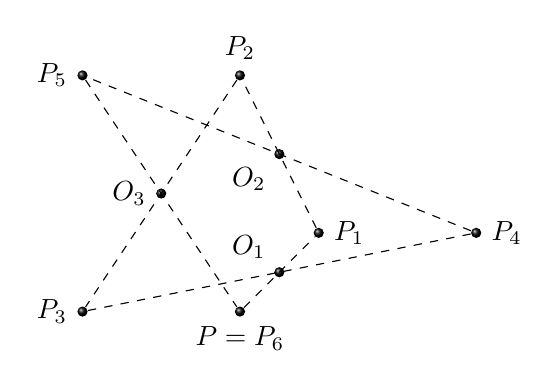
\begin{tikzpicture}
\begin{scope}[scale=0.5]
    %points
    \node[ball,label={below:$P=P_6$}] (p) at (0, -3) {};
    \node[ball,label={above left:$O_1$}] (o1) at (1, -2) {};
    \node[ball,label={below left:$O_2$}] (o2) at (1, 1) {};
    \node[ball,label={left:$O_3$}] (o3) at (-2, 0) {};
    \node[ball,label={right:$P_1$}] (p1) at (2, -1) {};
    \node[ball,label={above:$P_2$}] (p2) at (0, 3) {};
    \node[ball,label={left:$P_3$}] (p3) at (-4, -3) {};
    \node[ball,label={right:$P_4$}] (p4) at (6, -1) {};
    \node[ball,label={left:$P_5$}] (p5) at (-4, 3) {};
    %lines
    \draw[dashed] (p) to (p1);
    \draw[dashed] (p1) to (p2);
    \draw[dashed] (p2) to (p3);
    \draw[dashed] (p3) to (p4);
    \draw[dashed] (p4) to (p5);
    \draw[dashed] (p5) to (p);
\end{scope}
\end{tikzpicture}
\end{document}
        \caption{Sequence of reflections across $O_1, O_2, O_3$}
    \end{figure}
    
    \begin{proof}
    A central symmetry about a point $O$ is equivalent to a rotation of $\pi$ radians around the same point $O$. Hence, we can consider three central symmetries, $R_{O_1}^{\pi}, R_{O_2}^{\pi}, R_{O_3}^{\pi}$. We know from lecture 2.2 that
    \[R_{O_1}^{\theta_1}\circ R_{O_2}^{\theta_2}=
    \begin{cases}
        R_{O_3}^{\theta_3} & \theta_1+\theta_2 \neq 2\pi k\\
        T_{\overrightarrow{v}} & \theta_1+\theta_2 = 2\pi k.
    \end{cases}\]
    \par Thus, $R_{O_1}^{\pi}\circ (R_{O_2}^{\pi}\circ R_{O_3}^{\pi})=R_{O_1}^{\pi}\circ T_{\overrightarrow{v}}$.
    \par We know from \ref{5a} that the composition of a central symmetry and a parallel transport is a central symmetry, so $R_{O_1}^{\pi}\circ T_{\overrightarrow{v}}=R_{O_4}^{\pi}$ for some fixed point $O_4$.
    \par Then for some point $p$, we have 
    \begin{align*}
        (R_{O_1}^{\pi}\circ (R_{O_2}^{\pi}\circ R_{O_3}^{\pi}))^2(p) 
        &=(R_{O_1}^{\pi}\circ T_{\overrightarrow{v}})^2(p)\\
        &=(R_{O_4}^{\pi})^2(p)\\
        &=\text{Id}(p)\\
        &=p.
    \end{align*}
    \end{proof}
    \item Consider three lines $a,b,c$ on the plane. Let $F=S_a\circ S_b\circ S_c$. Prove that $F\circ F$ is a parallel transport.
    
    \begin{figure}[ht]
        \centering
        \documentclass{standalone}
\usepackage{tikz}
%------------tikz Setup------------

\tikzstyle{ball} = [circle,shading=ball, ball color=black,
    minimum size=1mm,inner sep=1.3pt]
\tikzstyle{miniball} = [circle,shading=ball, ball color=black,
    minimum size=1mm,inner sep=0.5pt]
\tikzstyle{mminiball} = [circle,shading=ball, ball color=black,
    minimum size=0.6mm,inner sep=0.1pt]
\usetikzlibrary{arrows.meta}
\usetikzlibrary{angles, quotes}
\tikzset{>={Latex[length=2mm,width=1.5mm]}}
\tikzset{->-/.style={decoration={markings, mark=at position #1 with
  {\arrow{>}}},postaction={decorate}}}
\usetikzlibrary{decorations.pathmorphing}
\usetikzlibrary{decorations.pathreplacing}
\usetikzlibrary{arrows.meta,calc}
\usetikzlibrary{bending}
\usetikzlibrary{decorations.markings,shapes.geometric}
\tikzset{->-/.style={decoration={markings, mark=at position #1 with
  {\arrow{>}}},postaction={decorate}}}
\tikzset{-|-/.style={decoration={markings, mark=at position #1 with
  {\arrow{stealth}}},postaction={decorate}}}
\tikzset{movearrow/.style 2 args ={
        decoration={markings,
    mark= at position {#1} with {\arrow{#2}} ,
        },
        postaction={decorate}
    }
}


\begin{document}
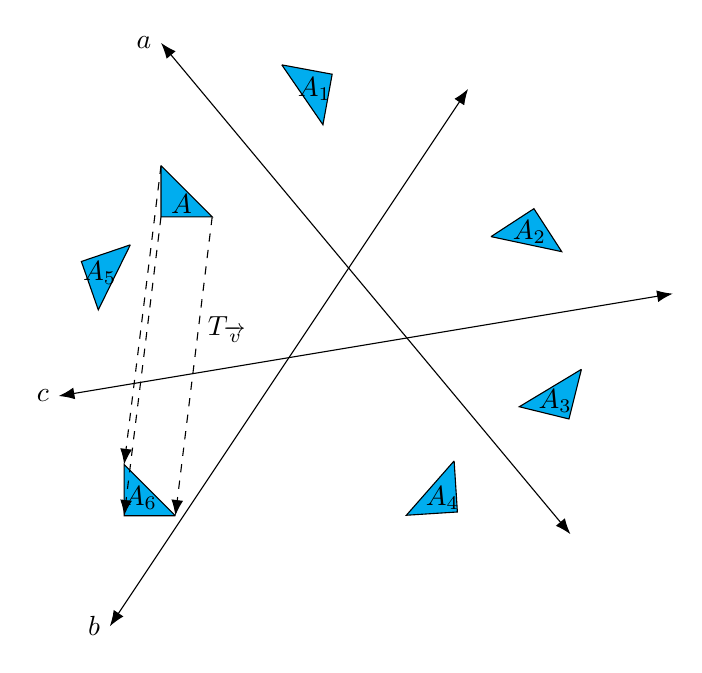
\begin{tikzpicture}
\begin{scope}[scale=0.65]
    %lines
    \draw[<->] (-4,4.4) -- (4,-5.2);
    \draw[<->] (-5,-7) -- (2,3.5);
    \draw[<->] (-6,-2.5) -- (6,-0.5);
    %line labels
    \node[left] (a) at (-4,4.4) {$a$};
    \node[left] (b) at (-5,-7) {$b$};
    \node[left] (c) at (-6,-2.5) {$c$};
    %triangles
    \draw[fill=cyan] (-4,2) -- (-3,1) -- (-4,1) -- (-4, 2);
    \draw[fill=cyan] (-1.64,3.97) -- (-0.836,2.8) -- (-0.656,3.787) -- (-1.64,3.97);
    \draw[fill=cyan] (2.448,0.614) -- (3.286,1.16) -- (3.83,0.32) -- (2.448,0.614);
    \draw[fill=cyan] (4.214,-1.979) -- (3.971,-2.949) -- (3,-2.71) -- (4.214,-1.979);
    \draw[fill=cyan] (1.727,-3.768) -- (1.791,-4.766) -- (0.794,-4.83) -- (1.727,-3.768);
    \draw[fill=cyan] (-4.6,0.453) -- (-5.225,-0.817) -- (-5.556,0.128) -- (-4.6,0.453);
    \draw[fill=cyan] (-3.72,-4.84) -- (-4.72,-3.84) -- (-4.72,-4.84) -- (-3.72,-4.84);
    %triangle labels
    \node(1) at (-3.6, 1.25) {$A$};
    \node(2) at (-1, 3.5) {$A_1$};
    \node(3) at (3.2, 0.7) {$A_2$};
    \node(4) at (3.7, -2.6) {$A_3$};
    \node(5) at (1.5, -4.5) {$A_4$};
    \node(6) at (-5.2, -0.1) {$A_5$};
    \node(7) at (-4.4, -4.5) {$A_6$};
    %vectors
    \draw[->,dashed] (-4,2) -- (-4.72,-3.84);
    \draw[->,dashed] (-3,1) -- (-3.72,-4.84);
    \draw[->,dashed] (-4,1) -- (-4.72,-4.84);
    \node(8) at (-2.7, -1.2) {$T_{\overrightarrow{v}}$};
\end{scope}
\end{tikzpicture}
\end{document}
        \caption{$F\circ F=(S_a\circ S_b\circ S_c)^2$}
    \end{figure}
    
    \begin{proof}
    By problem 3 of Problem Set 4, the composition of three reflections is a sliding symmetry. Therefore, we can let $F=S_d\circ T_{\overrightarrow{v}}=T_{\overrightarrow{v}}\circ S_d$ for some line $d$ and some vector $\overrightarrow{v}$. Thus,
    \[F\circ F=(T_{\overrightarrow{v}}\circ S_d)\circ (S_d\circ T_{\overrightarrow{v}})=T_{\overrightarrow{v}}\circ T_{\overrightarrow{v}}=T_{\overrightarrow{2v}}\]
    which is a parallel transport, as desired.
    \end{proof}
\end{enumerate}


\section{Problem 6.}
Prove that a bounded figure in $\mathbb{R}^2$ cannot have more than one center of symmetry. A bounded figure is any subset of $\mathbb{R}^2$, contained in sufficiently large disc.
\begin{proof}
Suppose there are two centers of symmetry, $A\neq B$. Then consider the line $\overleftrightarrow{AB}$, which must pass through two points on the figure, call them $P_1$ and $P_2$, since the figure is bounded. Then $|P_1A|=|AP_2|=\frac{|P_1P_2|}{2}$ and $|P_1B|=|BP_2|=\frac{|P_1P_2|}{2}$. Hence, $|P_1A|=|P_1B|$ and $|AP_2|=|BP_2|$. Since $A$ and $B$ are on the same side of $P_1$ and on the same side of $P_2$, we must have $A=B$.
\end{proof}


\section{Problem 7.}
Let S be a set with operation $\star: S\times S\rightarrow S$. Consider a number $A_n$ of ways to put brackets in an expression
\[a_1\star a_2\star ...\star a_{n+1}.\tag{1}\label{1}\]
For instance, $A_2=2$ because there are just two ways: $(a_1\star a_2)\star a_3$ and $a_1\star (a_2\star a_3)$.
\begin{enumerate}[label=(\alph*)]
    \item Compute $A_1,A_2,A_3,A_4$. \label{a}
    \begin{enumerate}[label=(\roman*)]
        \item $A_1=1$.
        \\$a_1 \star a_2.$
        \item $A_2=2$.
        \\$(a_1\star a_2)\star a_3.$
        \\$a_1\star (a_2\star a_3).$
        \item $A_3=5$.
        \\$(a_1 \star a_2) \star (a_3 \star a_4).$
        \\$((a_1 \star a_2) \star a_3) \star a_4.$
        \\$(a_1 \star (a_2 \star a_3)) \star a_4.$
        \\$a_1 \star ((a_2 \star a_3) \star a_4).$
        \\$a_1 \star (a_2 \star (a_3 \star a_4)).$
        \item $A_4=14$.
        \\$a_1 \star ((a_2 \star a_3) \star (a_4 \star a_5)).$
        \\$a_1 \star (((a_2 \star a_3) \star a_4) \star a_5).$
        \\$a_1 \star ((a_2 \star (a_3 \star a_4) \star a_5)).$
        \\$a_1 \star (a_2 \star ((a_3 \star a_4) \star a_5)).$
        \\$a_1 \star (a_2 \star (a_3 \star (a_4 \star a_5))).$
        \\$(a_1 \star a_2) \star ((a_3 \star a_4) \star a_5).$
        \\$(a_1 \star a_2) \star (a_3 \star (a_4 \star a_5)).$
        \\$((a_1 \star a_2) \star a_3) \star (a_4 \star a_5).$
        \\$(a_1 \star (a_2 \star a_3)) \star (a_4 \star a_5).$
        \\$((a_1 \star a_2) \star (a_3 \star a_4)) \star a_5.$
        \\$(((a_1 \star a_2) \star a_3) \star a_4) \star a_5.$
        \\$((a_1 \star (a_2 \star a_3)) \star a_4) \star a_5.$
        \\$(a_1 \star ((a_2 \star a_3) \star a_4)) \star a_5.$
        \\$(a_1 \star (a_2 \star (a_3 \star a_4))) \star a_5.$
    \end{enumerate}
    \item Prove that $A_n=A_0A_{n-1}+A_1A_{n-2}+...+A_{n-1}A_0$. Deduce that $A_n=c_n$. 
    \begin{proof}
    We know $A_0=1$ and $A_1=1$. We will proceed by strong induction.
    \par Base case. We have from \ref{a} that $A_2=A_0A_1+A_1A_0=1\times 1+1\times 1=2.$
    \par Inductive step. Assume that the recursive formula holds for $1,2,\dots, n-1$. Then we can show that $A_n=A_0A_{n-1}+A_1A_{n-2}+...+A_{n-1}A_0$. We can analyze term by term. $A_iA_{n-1-i}$ first splits $a_1, a_2,\dots, a_{n+1}$ into two groups, $a_1,\dots,a_{i+1}$ and $a_{i+2},\dots,a_{n+1}$. By the inductive assumption, $A_i$ counts the number of ways to put brackets around the first group, and $A_{n-1-i}$ counts the number of ways to put brackets around the second. By the fundamental counting principle, $A_iA_{n-1-i}$ counts the total number of ways to put brackets around all elements for this grouping. Then,
    \[\sum_{i=0}^{n-1} A_iA_{n-1-i}=A_0A_{n-1}+A_1A_{n-2}+...+A_{n-1}A_0=A_n.\]
    represents the total number of ways to put brackets around all elements in all groupings.
    \par Thus, the recursive formula for $A_n$ is the same as the recursive formula for $c_n$, and $A_0=c_0=A_1=c_1=1$, so $A_n=c_n$ for every $n$.
    \end{proof}
    \item Find an explicit bijection between ways to put brackets in \eqref{1} and triangulations of a convex $(n+2)-$gon.
    \par Triangulations to brackets. Start by labelling the sides in order from $a_1$ to $a_{n+1}$, leaving one side unlabelled. Then, for each triangle, if two sides are labelled, then write the product of the two sides in brackets and label the third side with this product. Eventually, the final bracketed expression will appear on the side of the $(n+2)-$gon that originally had no label.
    
    \begin{figure}[ht]
        \centering
        \documentclass{standalone}
\usepackage{tikz}
%------------tikz Setup------------

\tikzstyle{ball} = [circle,shading=ball, ball color=black,
    minimum size=1mm,inner sep=1.3pt]
\tikzstyle{miniball} = [circle,shading=ball, ball color=black,
    minimum size=1mm,inner sep=0.5pt]
\tikzstyle{mminiball} = [circle,shading=ball, ball color=black,
    minimum size=0.6mm,inner sep=0.1pt]
\usetikzlibrary{arrows.meta}
\usetikzlibrary{angles, quotes}
\tikzset{>={Latex[length=2mm,width=1.5mm]}}
\tikzset{->-/.style={decoration={markings, mark=at position #1 with
  {\arrow{>}}},postaction={decorate}}}
\usetikzlibrary{decorations.pathmorphing}
\usetikzlibrary{decorations.pathreplacing}
\usetikzlibrary{arrows.meta,calc}
\usetikzlibrary{bending}
\usetikzlibrary{decorations.markings,shapes.geometric}
\tikzset{->-/.style={decoration={markings, mark=at position #1 with
  {\arrow{>}}},postaction={decorate}}}
\tikzset{-|-/.style={decoration={markings, mark=at position #1 with
  {\arrow{stealth}}},postaction={decorate}}}
\tikzset{movearrow/.style 2 args ={
        decoration={markings,
    mark= at position {#1} with {\arrow{#2}} ,
        },
        postaction={decorate}
    }
}


\begin{document}
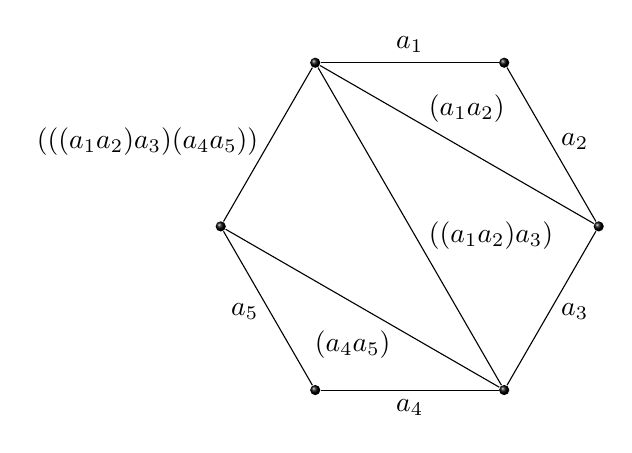
\begin{tikzpicture}
\begin{scope}[scale=1.2]
    %vertices
    \node[ball] (1) at (-1, 1.732) {};
    \node[ball] (2) at (1, 1.732) {};
    \node[ball] (3) at (2, 0) {};
    \node[ball] (4) at (1, -1.732) {};
    \node[ball] (5) at (-1, -1.732) {};
    \node[ball] (6) at (-2, 0) {};
    %edges
    \draw (1) to (2);
    \draw (2) to (3);
    \draw (3) to (4);
    \draw (4) to (5);
    \draw (5) to (6);
    \draw (6) to (1);
    %triangulations
    \draw (1) to (3);
    \draw (1) to (4);
    \draw (6) to (4);
    %labels
    \node[above] at (0,1.732) {$a_1$};
    \node[right] at (1.5,0.9) {$a_2$};
    \node[above right] at (0.1,1) {$(a_1a_2)$};
    \node[right] at (1.5,-0.9) {$a_3$};
    \node[right] at (0.1,-0.1) {$((a_1a_2)a_3)$};
    \node[below] at (0,-1.732) {$a_4$};
    \node[left] at (-1.5,-0.9) {$a_5$};
    \node[below left] at (-0.1,-1) {$(a_4a_5)$};
    \node[left] at (-1.5,0.9) {$(((a_1a_2)a_3)(a_4a_5))$};
\end{scope}
\end{tikzpicture}
\end{document}
        \caption{One map between triangulations and brackets for $n=4$}
    \end{figure}

    \par Brackets to triangulations. Start by labelling the sides in order from $a_1$ to $a_{n+1}$, leaving one side unlabelled. Start by locating pairs $(a_ia_{i+1})$ in the bracketed expression and draw lines to form a triangle with $a_i$ and $a_{i+1}$, labelling the new line with $(a_ia_{i+1})$. We can proceed by doing the same with larger expressions. Let $(x)$ and $(y)$ be bracketed expressions, then draw a line to create a triangle between sides labelled $(x)$ and $(y)$ if $((x)(y))$ is in the bracketed expression.
\end{enumerate}


\section{Problem 8. Sylvester’s theorem}
Consider $n$ lines in the plane, not all of which pass through the same point. The lines are not all parallel. Prove that there exists a point in which exactly two of the lines intersect.
\begin{proof}
Let us prove the following dual statement: Let a finite set $S$ of points lie in the plane such that they are not all co-linear. Then there is a line that passes through exactly two of the points.
\par For each line $\ell_i$ that passes through at least two points in $S$, let $d(p_i, \ell_i)$ be the perpendicular distance from each point $p_i$ to $\ell_i$. Suppose there exists a point $p$ and line $\ell$ such that $d$ is minimized, and let $p'$ be the perpendicular projection of $p$ onto $\ell$. We will show that $\ell$ passes through exactly two points in $S$ by contradiction.

\begin{figure}[ht]
    \centering
    \documentclass{standalone}
\usepackage{tikz}
%------------tikz Setup------------

\tikzstyle{ball} = [circle,shading=ball, ball color=black,
    minimum size=1mm,inner sep=1.3pt]
\tikzstyle{miniball} = [circle,shading=ball, ball color=black,
    minimum size=1mm,inner sep=0.5pt]
\tikzstyle{mminiball} = [circle,shading=ball, ball color=black,
    minimum size=0.6mm,inner sep=0.1pt]
\usetikzlibrary{arrows.meta}
\usetikzlibrary{angles, quotes}
\tikzset{>={Latex[length=2mm,width=1.5mm]}}
\tikzset{->-/.style={decoration={markings, mark=at position #1 with
  {\arrow{>}}},postaction={decorate}}}
\usetikzlibrary{decorations.pathmorphing}
\usetikzlibrary{decorations.pathreplacing}
\usetikzlibrary{arrows.meta,calc}
\usetikzlibrary{bending}
\usetikzlibrary{decorations.markings,shapes.geometric}
\tikzset{->-/.style={decoration={markings, mark=at position #1 with
  {\arrow{>}}},postaction={decorate}}}
\tikzset{-|-/.style={decoration={markings, mark=at position #1 with
  {\arrow{stealth}}},postaction={decorate}}}
\tikzset{movearrow/.style 2 args ={
        decoration={markings,
    mark= at position {#1} with {\arrow{#2}} ,
        },
        postaction={decorate}
    }
}


\begin{document}
\begin{tikzpicture}
\begin{scope}[scale=2.5]
    %nodes
    \node[ball,label={above:$p$}] (p) at (0, 1) {};
    \node[ball,label={below:$p'$}] (p') at (0, 0) {};
    \node[ball,label={below:$a$}] (a) at (1, 0) {};
    \node[ball,label={below:$b$}] (b) at (2, 0) {};
    \node[ball,label={above:$a'$}] (a') at (1.2, 0.4) {};
    %right angles
    \draw (0,0.13) -- (0.13,0.13) -- (0.13, 0);
    \draw (1.14,0.3) -- (1.25,0.25) -- (1.3, 0.35);
    %lines
    \draw [<->] (-0.5,0) -- (2.5, 0);
    \node[left] at (-0.5,0) {$\ell$};
    \draw [dashed] (a) -- (a');
    \node[left] at (0.8,0.8) {$m$};
    %projections
    \draw [dashed] (p) -- (p');
    \draw [<->, dashed] (p) -- (b);
\end{scope}
\end{tikzpicture}
\end{document}
    \caption{Sylvester's theorem}
\end{figure}

\par Assume that $S$ passes through at least three points in $S$. Then at least two of these, call them $a$ and $b$, lie on the same side of $p'$, with $a$ possibly coinciding with $p'$. Draw the line $m$ passing through $p$ and $b$, and let $a'$ be the perpendicular projection of $a$ onto $m$. Then $d(a,m)<d(p,\ell )$ since $\triangle bp'p\sim \triangle ba'a$, which contradicts our original assumption that $p$ and $\ell$ minimizes $d$.
\par Thus, a line that passes though exactly two of the points exists, as desired.
\end{proof}


\end{document}
